\documentclass{llncs}
\usepackage{graphicx}
% please place your own definitions here and don't use \def but
\newcommand{\middot}{\ensuremath{\cdot\:}}
%
\begin{document}

\title{A Flexible Laboratory Environment Supporting Honeypot Deployment for 
Teaching Real-World Cybersecurity Skills
%\thanks{Grants or other notes
%about the article that should go on the front page should be
%placed here. General acknowledgments should be placed at the end of the article.}
}
%\subtitle{Do you have a subtitle?\\ If so, write it here}

%\titlerunning{Honeypots in H.E. teaching}        % if too long for running head

\author{Neil~Eliot \and David~Kendall \and Michael~Brockway}

%\authorrunning{Short form of author list} % if too long for running head

\institute{Northumbria University \\ \email{neil.eliot@northumbria.ac.uk}}

%\date{Received: date / Accepted: date}
% The correct dates will be entered by the editor


\maketitle

\begin{abstract}
  Teaching cybersecurity within a University environment requires a closed
  environment that is off-campus and configured such that students can transfer
  theoretical principles into practical cybersecurity skills. The subject
  necessitates the need for honeypot technologies that will allow the
  investigation of network-based cybersecurity attacks. The need for a closed
  environment, which may be considered as a ``sandbox'', arises from the nature
  of cybersecurity investigations, especially where students are required to
  investigate network protocol-based attacks that could render a teaching
  network environment unstable or unusable.

  Although the environments are closed they still require access to the Internet.
  The honeypot platform and the teaching environments discussed in this paper
  are designed so as to provide an environment that is flexible enough to allow
  the teaching of general purpose networking and operating systems subjects,
  and to support complex sand-boxed integration of honeypot technologies for
  the teaching of the practical aspects of cybersecurity.

  The paper concludes by outlining how the platform has been successfully
  deployed within a University environment to support undergraduate and
  postgraduate teaching and learning by highlighting the types of
  experimentation and projects that the environment has supported and will
  support in the future.
  \keywords{Cyber Security \middot\ Network Security \middot\ Honeypot \middot\ Teaching}
\end{abstract}


\section{Introduction}\label{intro}
When teaching cybersecurity in an academic environment there are many
considerations that need to be taken into account, not least, respecting other
users privacy and their access to the learning and teaching facilities within
the academic environment.

Activities such as reconnaissance and experimentation can result in traffic or
services being deployed into the teaching network environment. These activities
may effect other users through service depletion, traffic
redirection~\cite{ACGO:06,LR:06} or through data capture that may compromise a
users legal rights e.g.\ capturing activity or sensitive information that you
are not authorised to possess.

The environment must also support activities that would normally be prevented
through configurations designed for production environments. A \emph{normal}
academic infrastructure designed for general student access may implement
restrictions through \texttt{MAC} blocking to prevent rogue equipment being
attached to the network or firewalls to prevent access to to specific Internet
sites. From a cybersecurity teaching perspective this would severely limit the
scope of the technologies that could be deployed and investigated and limit
access to potential teaching resources~\cite{ACGO:06,YYLCHJ:04}. Also a general
purpose network deployment would not provide students with the administrative
privileges that are required.

When investigating cybersecurity there is also a need for the environment to
be controlled such that the services and network protocols are minimised or
reduced  therefore the effects an attack have upon the environment can be
isolated and analyses effectively i.e.\ if analysing the effects of throughput
on a protocol any rogue activities, such as file transfers or service
advertising may impact on the experimental environment and invalidate the
results.

These issues highlight the need for a clear definition of the requirements of
\emph{academic honeypot} environments and the need for closed specialist
environments for the study of cybersecurity.

Honeypots are computer systems that are specifically designed for
cybersecurity investigations~\cite{FKAS:17,BCF:12,ZZQL:03}. They may be
implemented as full network deployments, incorporating switches, routers, and
multiple servers providing network services, or they may be implemented as a
program running on a single machine. 

Honeypots can be classified in terms of the level of interaction and
analysis that they offer, and also in terms of the volume of concurrent requests
that they may be required to process.

\begin{itemize}

  \item \noindent \emph{\textbf{Low Interaction:}} Implements coarse-grained
    services and captures only a low-level of detail about their implementation
    and their interaction with users.  This type of honeypot can also be used
    to act as an attractor for bot-based attacks~\cite{SZB:16}.  

  \item \noindent \emph{\textbf{High Interaction:}} Implements fine-grained
    services and captures a high-level of detail about their implementation and
    their interaction with users.  This type of honeypot is called a
    ``research'' honeypot by Mairh et al.~\cite{MBVJ:11}. High-interaction
    honeypots can also be used to distract potential hackers from a genuine
    system (a decoy)~\cite{M:06,SNKA:12}.

\end{itemize}


\begin{itemize}

  \item \noindent \emph{\textbf{Low Volume:}} Capable of supporting only a
    small number of concurrent requests.  This type honeypot is often deployed
    in a research or teaching laboratory to investigate the details of a single
    attack type.

  \item \noindent \emph{\textbf{High Volume:}} Capable of supporting a large
    number of concurrent requests. This type of honeypot is often deployed in
    an environment that results in the honeypot being subjected to high levels
    of usage from multiple sources. 

\end{itemize}

These two categories provide four different types of honeypot based upon
interaction and volume. We use the obvious acronyms to refer to each different
type, as shown in Table~\ref{table:HoneypotTypes}.

\begin{table}[h]
\caption{Honeypot types by interaction and volume\label{table:HoneypotTypes}}
\begin{center}
\begin{tabular}{| c | c| c |}
\hline
 & Low Volume & High Volume \\
\hline
Low Interaction & \texttt{LILV} & \texttt{LIHV} \\
\hline
High Interaction & \texttt{HILV} & \texttt{HIHV} \\
\hline
\end{tabular}
\end{center}
\end{table}

This paper focuses on \emph{L}ow-\emph{I}nteraction-\emph{H}igh-\emph{V}olume
(\texttt{LIHV}) and \emph{H}igh-\emph{I}nteraction-\emph{L}ow-\emph{V}olume
(\texttt{HILV}) honeypots and the requirements of an academic networking
platform to support their use in the delivery of both undergraduate and
postgraduate cybersecurity programmes.

The two other types of honeypot are not required for undergraduate purposes.
\emph{L}ow-\emph{I}nteraction-\emph{L}ow-\emph{V}olume (\texttt{LILV})
honeypots have limited utility and, if required,  can be deployed inside the
\texttt{HILV} platform, for example as an academic exercise in installing and
testing a tool such as Kippo~\cite{D:16,SH:15}.
\emph{H}igh-\emph{I}nteraction-\emph{H}igh-\emph{V}olume (\texttt{HIHV})
honeypots are expensive to deploy and time-consuming to reconfigure for
different teaching scenarios. This type of honeypot would be useful in a
research environment such as a research centre for use in long term
Internet-based projects. 

\paragraph{Related Work.}
Romney and Lanoy~\cite{LR:06} discuss the use of virtual environments as a
mechanism to deploy honeypot platforms, virtualisation as a technology can
introduce limitations with respect to deployment, resource utilisation, and
data capture. Aspects of the deployment discussed in this paper are similar to
those of Romney and Lanoy but the focus in this paper is the use of honeypots
for undergraduate and post-graduate students. The paper extends their work by
deploying honeypot environments as a physical configuration to increase the
potential use of the honeypots as a learning environment. Spitner~\cite{LS:03}
discusses many cybersecurity based attack techniques and the physically
deployed \texttt{HILV} lends itself to the types of attacks he discusses. This
includes deploying a \texttt{HILV} honeypot within the laboratory and allowing
access from the laboratory to specific services or equipment within it to
emulate ``real'' attacks.

The honeypot designs in this paper extend the ability to deploy multi-honeypot
experimental environments as discussed by Duffany~\cite{JD:08}. This is
achieved by reducing the cost of the honeypot architecture to increase the
number of available honeypots for a distributed data capture deployment. The
proposals in this paper also make the \texttt{LIHV} honeypot architecture small
enough to be a portable device suitable for deployment in multiple locations.

\section{Teaching Requirements}\label{sec:TeachingRequire}

\subsection{General Networking Laboratory}\label{subsec:GeneralLab}

\subsubsection{Requirement 1.} 
There must be a flexible re-configurable base laboratory environment, isolated
from the main university campus network, for students to carry out their normal
studies of networks, operating systems and network services. Students require
administrative access to the basic networking equipment such as routers,
switches, and desktop machines for installation and configuration of general
purpose tools and virtual environments. These activities would normally be
prohibited on a University campus network. It should be possible to quickly
restore a standard software environment to all devices.

\subsubsection{Requirement 2.}
The laboratory network should implement a security policy, independent of the
standard University policy, controlling access to the Internet. This is to
allow students to access security sites and relevant software packages. Many
academic networks block access to cybersecurity tool sites from their
specialist and general access laboratories~\cite{ACGO:06,YYLCHJ:04}, as well as
from the open access areas used by students. Tools such a
\texttt{Metasploit}~\cite{R7:17} or the \texttt{Kali Linux}
distribution~\cite{OS:17} are usually blocked, as are cybersecurity information
sites such as \texttt{http://www.hak5.org} or
\texttt{https://www.exploit-db.com/}. It must be possible to lift these
restrictions in a laboratory supporting cybersecurity studies.

\subsection{\texttt{LIHV} Honeypot}\label{subsec:LabHoneypot}

\subsubsection{Requirement 3.} 
There needs to be a facility that allows large numbers of students to test
existing cybersecurity tools and to provide them with the ability to develop
and test their own tools.

\subsection{\texttt{HILV} Honeypot}\label{subsec:ResearchHoneypot}

\subsubsection{Requirement 4.} 
The \texttt{HILV} honeypot must allow students: to deploy basic networking services
on multiple low-cost servers
(e.g.\ \texttt{DHCP}/\texttt{DNS}/\texttt{HTTP}/\texttt{DB}); to attack these
services; and to capture and analyse the details of the network traffic
and server events that are generated.

\subsubsection{Requirement 5.} 
In order to satisfy Requirement 4, while protecting the rest of the laboratory
from the effects of attacks, there needs to be a mechanism that allows students
to connect their servers to the general networking laboratory via port mapping
or address forwarding.

\subsubsection{Requirement 6.} 
The servers need to have limited hardware resources in order to allow the
analysis of resource exhaustion attacks without requiring a large number of
attacking end points, e.g.\ it should be possible to launch a successful
resource exhaustion attack from a botnet consisting of a few machines rather
than hundreds or thousands.

\subsubsection{Requirement 7.} 
The honeypot must provide scope for additional services and devices to be
added. It must also provide the ability to cascade multiple honeypots to create
a honeynet~\cite{AA:15,FDF:15,KNC:15}.

\subsubsection{Requirement 8.} 
The honeypot must facilitate effective network traffic capture to ensure the
integrity of any network analysis e.g.\ identifying network transactions in a
website defacement or denial of service-based (\texttt{DoS} or \texttt{DDoS})
attack, or spoofed packets such as in \texttt{ARP} poisoning for
man-in-the-middle (\texttt{MitM}) attacks~\cite{PS:16,RSKA:16}.

\section{Logical/Physical Network Infrastructure}\label{LogicalDesign}

The teaching environment consists of three distinct components: The general
networking laboratory (\textit{requirement 1,2}), the \texttt{LIHV} honeypot
(\textit{requirement 3}) and the small scale \texttt{HILV} honeypots
(\textit{requirements 4,5,6,7,8}).

\subsection{General Networking Laboratory}

The flexible laboratory environment needs to provide a re-configurable physical
networking layer. This is provided by a structured cabling architecture as
shown in~Fig.~\ref{fig:Overview1}.

\begin{figure}[h]
\begin{center}
	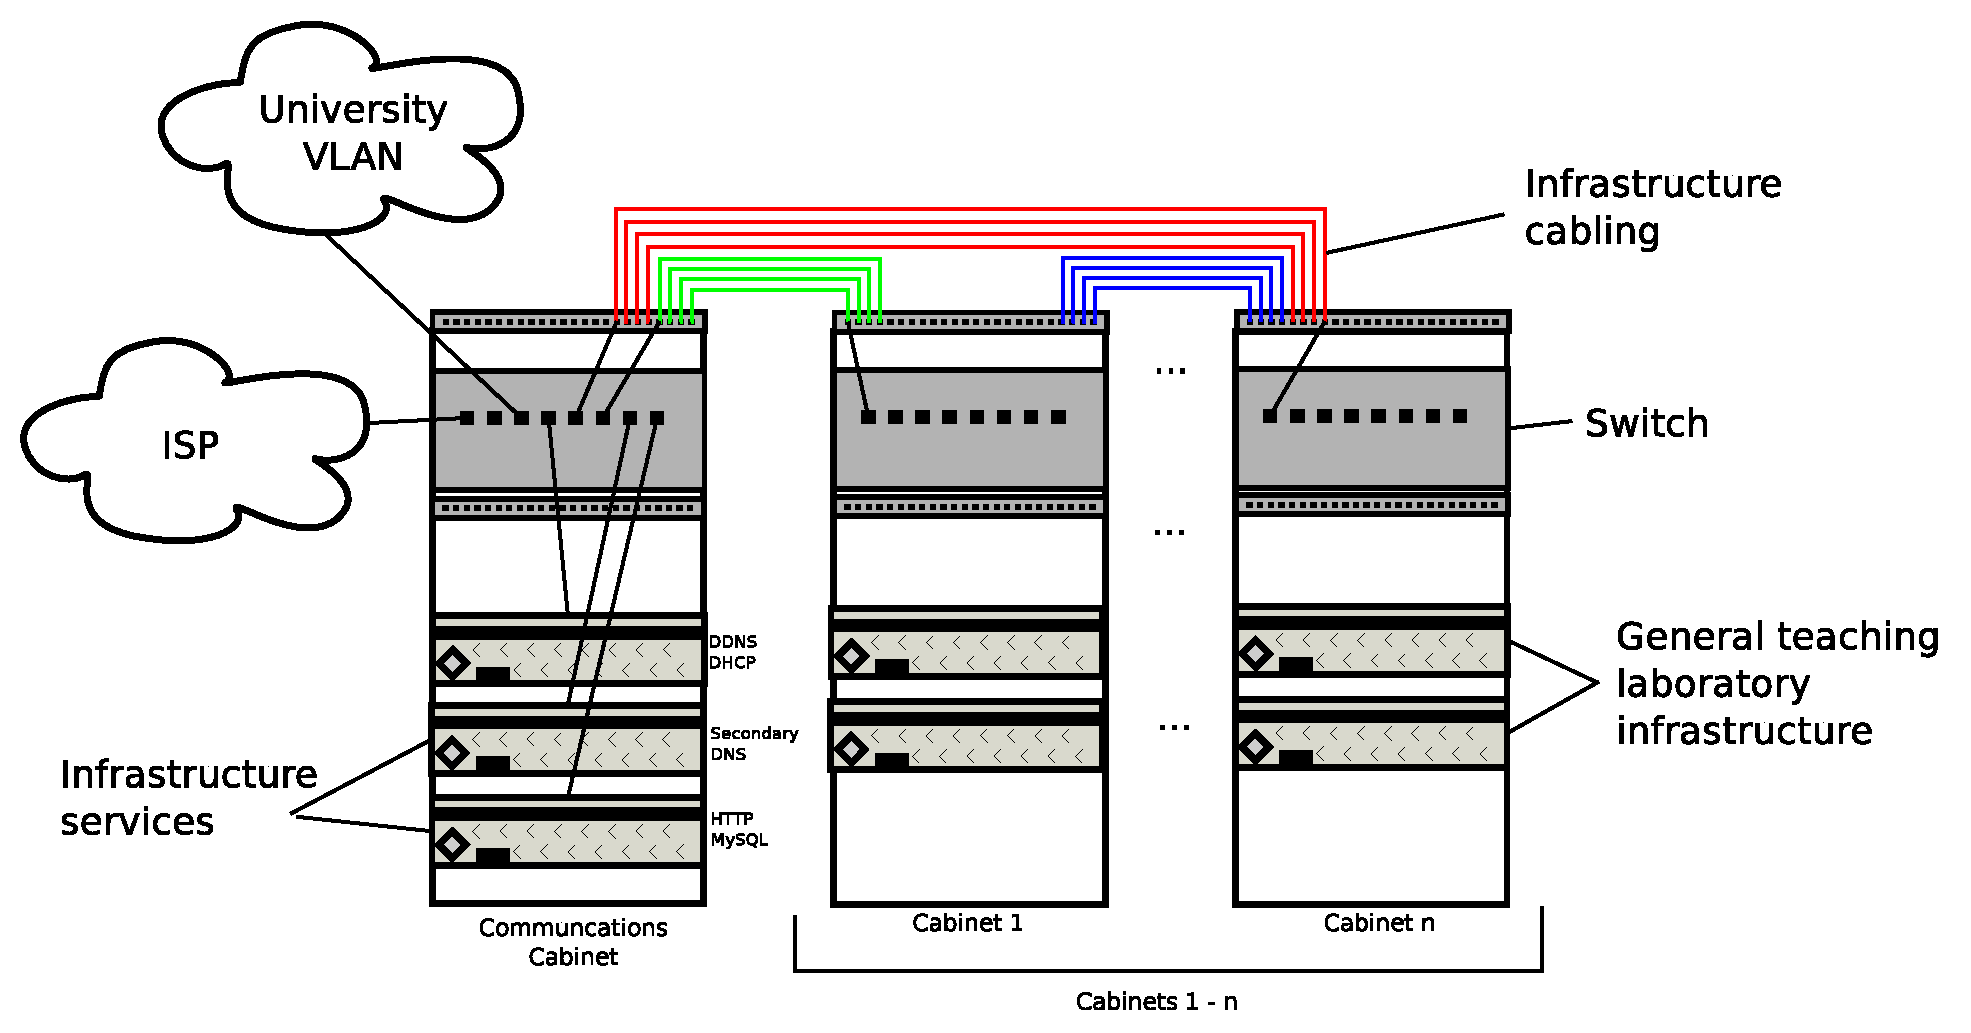
\includegraphics[scale=0.4]{Images/Infrastructure.eps}
\caption{General networking laboratory overview}
\label{fig:Overview1}
\end{center}
\end{figure}

The ``Communications Cabinet'' is secured; students are not allowed access, to
prevent reconfiguration of the base network and the network services equipment.
The cabinet contains the \texttt{DHCP} and \texttt{DNS} servers, a 1U intranet
server, a database server and a \texttt{NAS} drive. The communication cabinet
includes a \texttt{VDSL} fibre link from the \texttt{ISP}. In the case of
Northumbria University the provider is BT Business~\cite{BT:17}. The router
used to manage the \texttt{ISP} connection is a Draytek Vigor
2850~\cite{DC:17}.

Each of the cabinets are linked to a laboratory bench supporting 8--10
students. Each cabinet contains a selection of switches, routers, \texttt{IP}
Telephony, \texttt{IDS}, and Firewall equipment that are required for general
network architecture modules. These cabinets are linked back to the
communications cabinet to provide Internet access for the benches. Access to
the Internet from the desktop is achieved through a \texttt{NAT} connection
from the communications cabinet \texttt{ISP} router.

The structured cabling allows the resources of each cabinet within the
laboratory to be linked to the desktop through four structured cabling ports.
Cross-cabinet connections ensure specialist resources are flexibly available to
all benches e.g.\ switches, routers, firewalls, and \texttt{IDS} (Intrusion
Detection Systems) etc.

\subsection{Address Range Support}

The use of virtualisation (\texttt{GNS3}~\cite{GNS3:17},
VMWare~\cite{VMWARE:17} and VirtualBox~\cite{O:17}) to support the operating
systems and networking modules necessitates a large number of host addresses,
to support a large number of students deploying statically addressed virtual
hosts. Running the base infrastructure as a single subnet allows freedom of
movement of the laboratory equipment. Using a class B address provides 65,534
addresses which is enough for each student to be allocated a block of
contiguous \texttt{IP} addresses for each module allowing multiple modules to
be delivered concurrently without having \texttt{IP} address conflicts.

\subsection{Network Service Deployment}\label{InfraService}

To support the operating systems and general computing subjects the network
requires, as a minimum, \texttt{DNS}~\cite{RA:11} and
\texttt{DHCP}~\cite{DL:02} services. These services two services are deployed
across three small scale 1U servers (HPE ProLiant DL360 Gen9
Server~\cite{HPE:17}). Two servers are located in the communications cabinet as
shown in~Fig.~\ref{fig:Overview1}. One server supports \texttt{DHCP} and
\texttt{DNS} which are integrated to create a \texttt{DDNS}~\cite{SV:06}
environment. The second server acts as the secondary \texttt{DNS} server. The
third server is located in the \texttt{LIHV} honeypot cabinet and acts as a
further secondary \texttt{DNS} server.

The communication cabinet also contains a 1U server that provides the
laboratory intranet (\texttt{LAMP} based) service, along with a general purpose
\texttt{MySQL} database services for the intranet and module content delivery.

Deployment of known desktop equipment is coordinated by creating reservation
entries in the \texttt{DHCP} service. The \texttt{DHCP} server then
automatically creates the forward and reverse \texttt{DNS} entries in the
\texttt{DNS} architecture as the equipment boots. Students can also connect
their own devices which are allocated a network configuration from a
\texttt{DHCP} address pool.

\subsection{Teaching Facilities Support}

The teaching of the standard technologies such as switching and routing utilise
the physical equipment within the cabinets. The laboratory also supports
network virtualisation through \texttt{GNS3} which can be integrated with the
physical equipment when necessary. The teaching of the \texttt{OS} based
technologies is supported through the use of desktop virtualisation allowing
each student to have multiple client and server technologies running
simultaneously on a single machine. For large scale deployments, which is
required on some modules, the deployment of the virtual machines is across
several desktop machines. The large scale deployments require the
virtualisation software to support network card bridging to allow the virtual
machines to be ``physically'' connected to the laboratory infrastructure.
Subjects that require a laboratory ``search-by-name'' facility (\texttt{DNS} and
\texttt{rDNS}) such as Java Sockets and C Sockets programming are supported by
the \texttt{DDNS} implementation as discussed in~Sect.~\ref{InfraService}.

\section{Honeypot Architectures}

As shown in Table~\ref{table:HoneypotTypes} the four types are:

\begin{itemize}
  \item \noindent \emph{\textbf{LIHV}} This type of honeypot is used when
    carrying out analysis of high levels of system interaction but only
    capturing a limited amount of service and system activity data for example
    analysing multiple attackers carrying out authentication attacks on an
    \texttt{FTP} server and only analysing the service log files. This type of
    honeypot can also be used in a general purpose networking laboratory with
    students to allow them to investigate authentication tools such as Hydra
    and xHydra~\cite{RS:15} and to be a target when they are developing their
    own tools such as an authentication based botnet.
  \item \noindent \emph{\textbf{LILV}} This type of honeypot is used when a
    basic testing platform is required to identify how a service is being
    attacked. There is no other interactions under investigation, for example
    using software systems such as Kippo~\cite{D:16,SH:15}, and testing how it
    logs transactions to a file or a database. There are a few login
    transactions from a limited number (usually 1) user and a simple activity
    log of attempted logins.
  \item \noindent \emph{\textbf{HIHV}} This type of honeypot is used when a
    system is being thoroughly tested with high levels of user interaction
    (pressure testing) and involves large numbers of high power servers capable
    of supporting high levels of concurrent interactions. These honeypots
    provide detailed data capture capabilities of all the services and the
    inter-service interactions as well as system transactions e.g. \texttt{SQL}
    Queries and responses. They are usually deployed as a ``real'' system that
    is being penetration tested and they are often exposed to the Internet to
    analyses the effects of unsolicited attacks.
  \item \noindent \emph{\textbf{HILV}} This type of honeypot is used when there
    is a low level of interaction with the system but the data captured is fine
    grain. For example investigating an enumeration attack such as a
    \texttt{DNS} query. The detail of the information gathered from the
    enumeration is low activity i.e.\ a single \texttt{AXFR}~\cite{EL:10}
    query., However the effect of the query and the activity it generates
    within the system is collected in great details. Another example would be
    profiling a \texttt{Wordpress}~\cite{WP:17} site using
    \texttt{WPScan}~\cite{WT:17}.
\end{itemize}

The two types of honeypot deployed in the laboratory are
\emph{H}igh-\emph{I}nteraction-\emph{L}ow-\emph{V}olume (\texttt{HILV}) and the
\emph{L}ow-\emph{I}nteraction-\emph{H}igh-\emph{V}olume (\texttt{LIHV}).

\subsection{\texttt{HILV} Honeypot}

The \texttt{HILV} honeypot architecture is an isolated environment. This is
achieved by using a commercially available cable router that is connected to
the main laboratory infrastructure as shown in Fig.~\ref{fig:HPOverview}.

\begin{figure}[!ht]
\begin{center}
	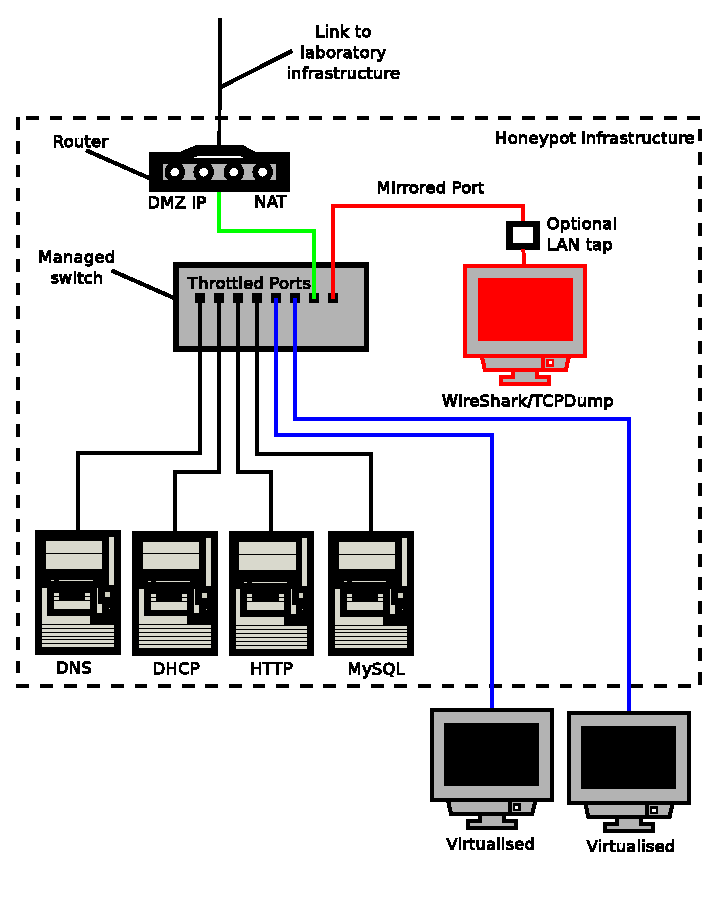
\includegraphics[scale=0.70]{Images/Honeypot1.eps}
\caption{\texttt{HILV} Honeypot overview}
\label{fig:HPOverview}
\end{center}
\end{figure}

Figures~\ref{fig:HP1}~and~\ref{fig:HP2} shows the complete device as deployed
in the specialist teaching laboratories. The complete research honeypot
consists of:

\begin{itemize}
    \item \noindent A router for traffic management to and from the laboratory
      infrastructure via \texttt{NAT} and Address forwarding. (connected via the
      green cable).  \item \noindent 4 Raspberry Pi boards for service deployment.
    \item \noindent A managed switch for packet capture:
    \begin{itemize}
        \item \noindent 1 port (port 8) setup as a monitor usually connected to
          a PC running TCPDump or Wireshark (Red Cable).
        \item \noindent All other ports are mirrored to the monitor (ports
          1--7).
        \item \noindent 1 port (port 7) links the switch and router.
        \item \noindent 4 ports (ports 1--4) are connected to the 4 Raspberry Pi 
        servers.
        \item \noindent 2 spare ports (ports 5,6) are available for additional
          services, clients, or devices to be added (Blue Cables).
    \end{itemize}
\end{itemize}

The two additional devices shown in Figure~\ref{fig:HPOverview} could be PCs to act as attack entry points or target devices such as PCs or wireless access points. These devices could also be PCs supporting virtualisation to extend the honeypot's functionality. Table~\ref{table:HoneypotCosts} shows the approximate costs of the basic \texttt{HILV} without additional devices or the monitoring PC attached.

\begin{table}[h]
\caption{Approximate costs\label{table:HoneypotCosts}}
\begin{center}
\begin{tabular}{| l | r |}
\hline
Item & Cost (\pounds) \\
\hline
Switch & 100 \\
\hline
Router & 100 \\
\hline
Raspberry Pi Boards (x4) & 100 \\
\hline
Fabrication & 50 \\
\hline
Cabling & 25 \\
\hline
Power supplies & 50 \\
\hline
\textbf{Total} & \textbf{425} \\
\hline
\end{tabular}
\end{center}
\end{table}

\begin{figure}[ht]
  \centering
  \begin{minipage}[h]{0.45\textwidth}
    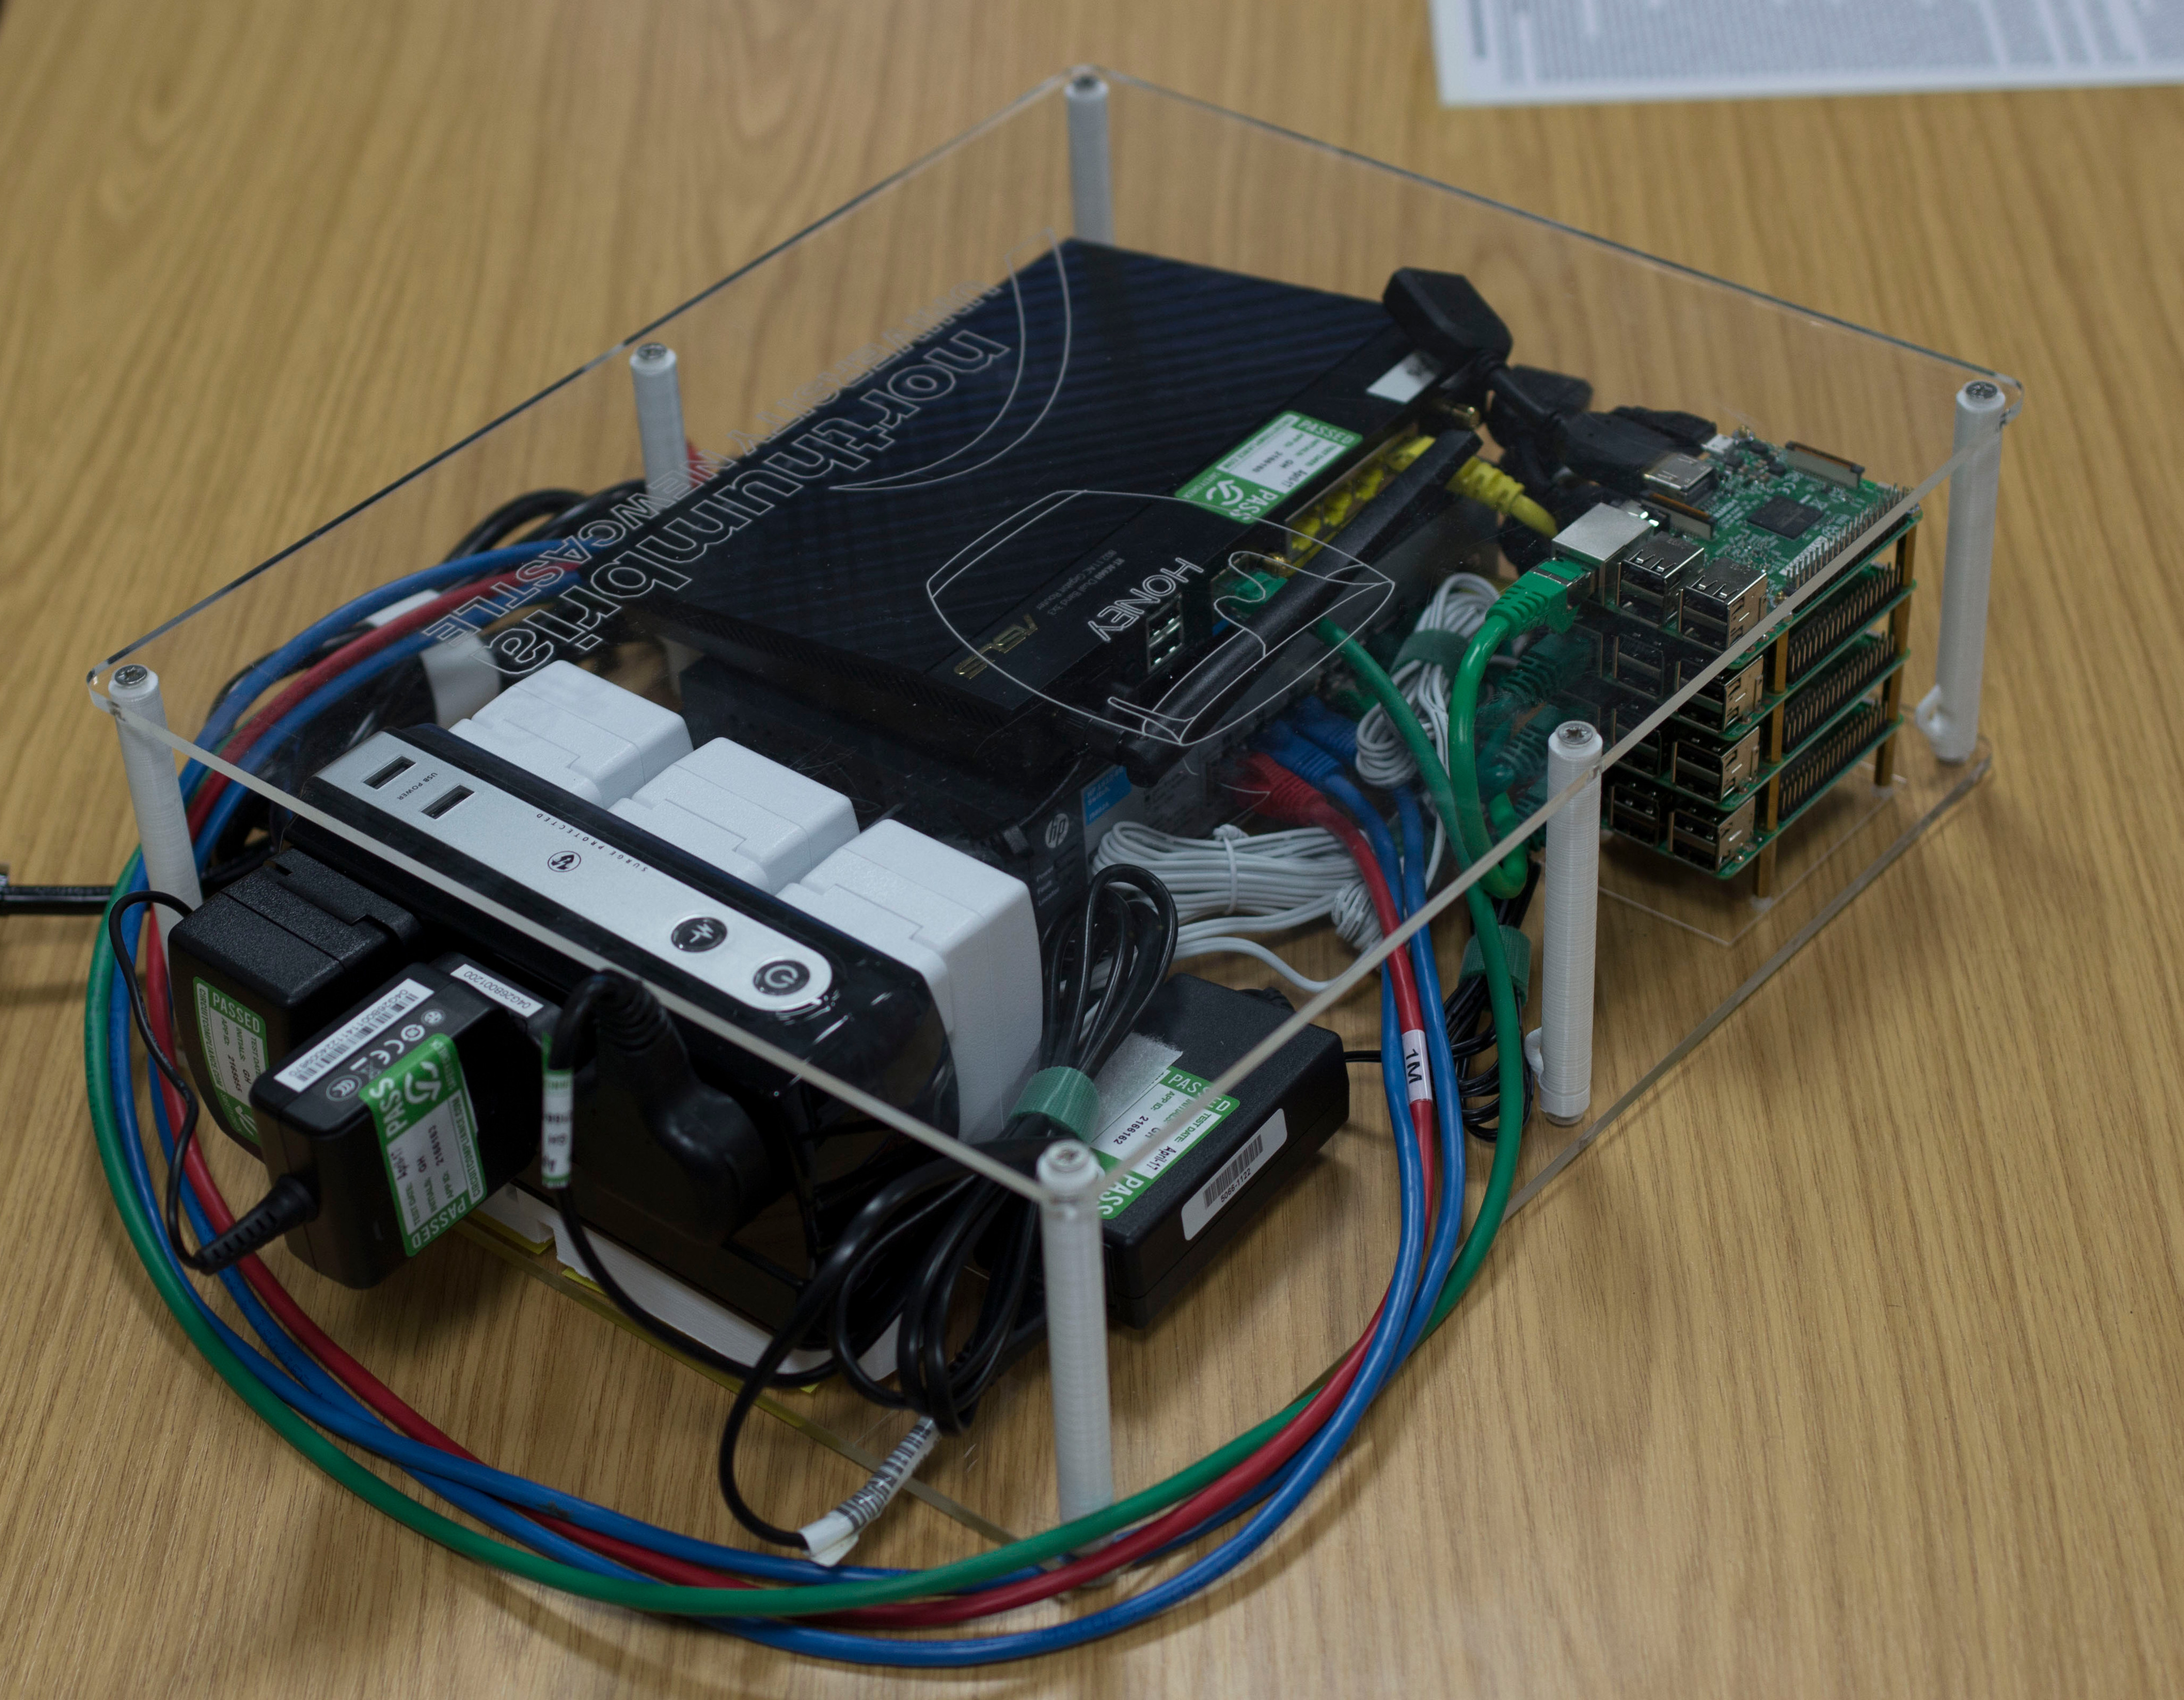
\includegraphics[width=\textwidth]{Images/HP1.eps}
    \caption{\texttt{HILV} side view\label{fig:HP1}}
  \end{minipage}
  \hfill
  \begin{minipage}[h]{0.45\textwidth}
    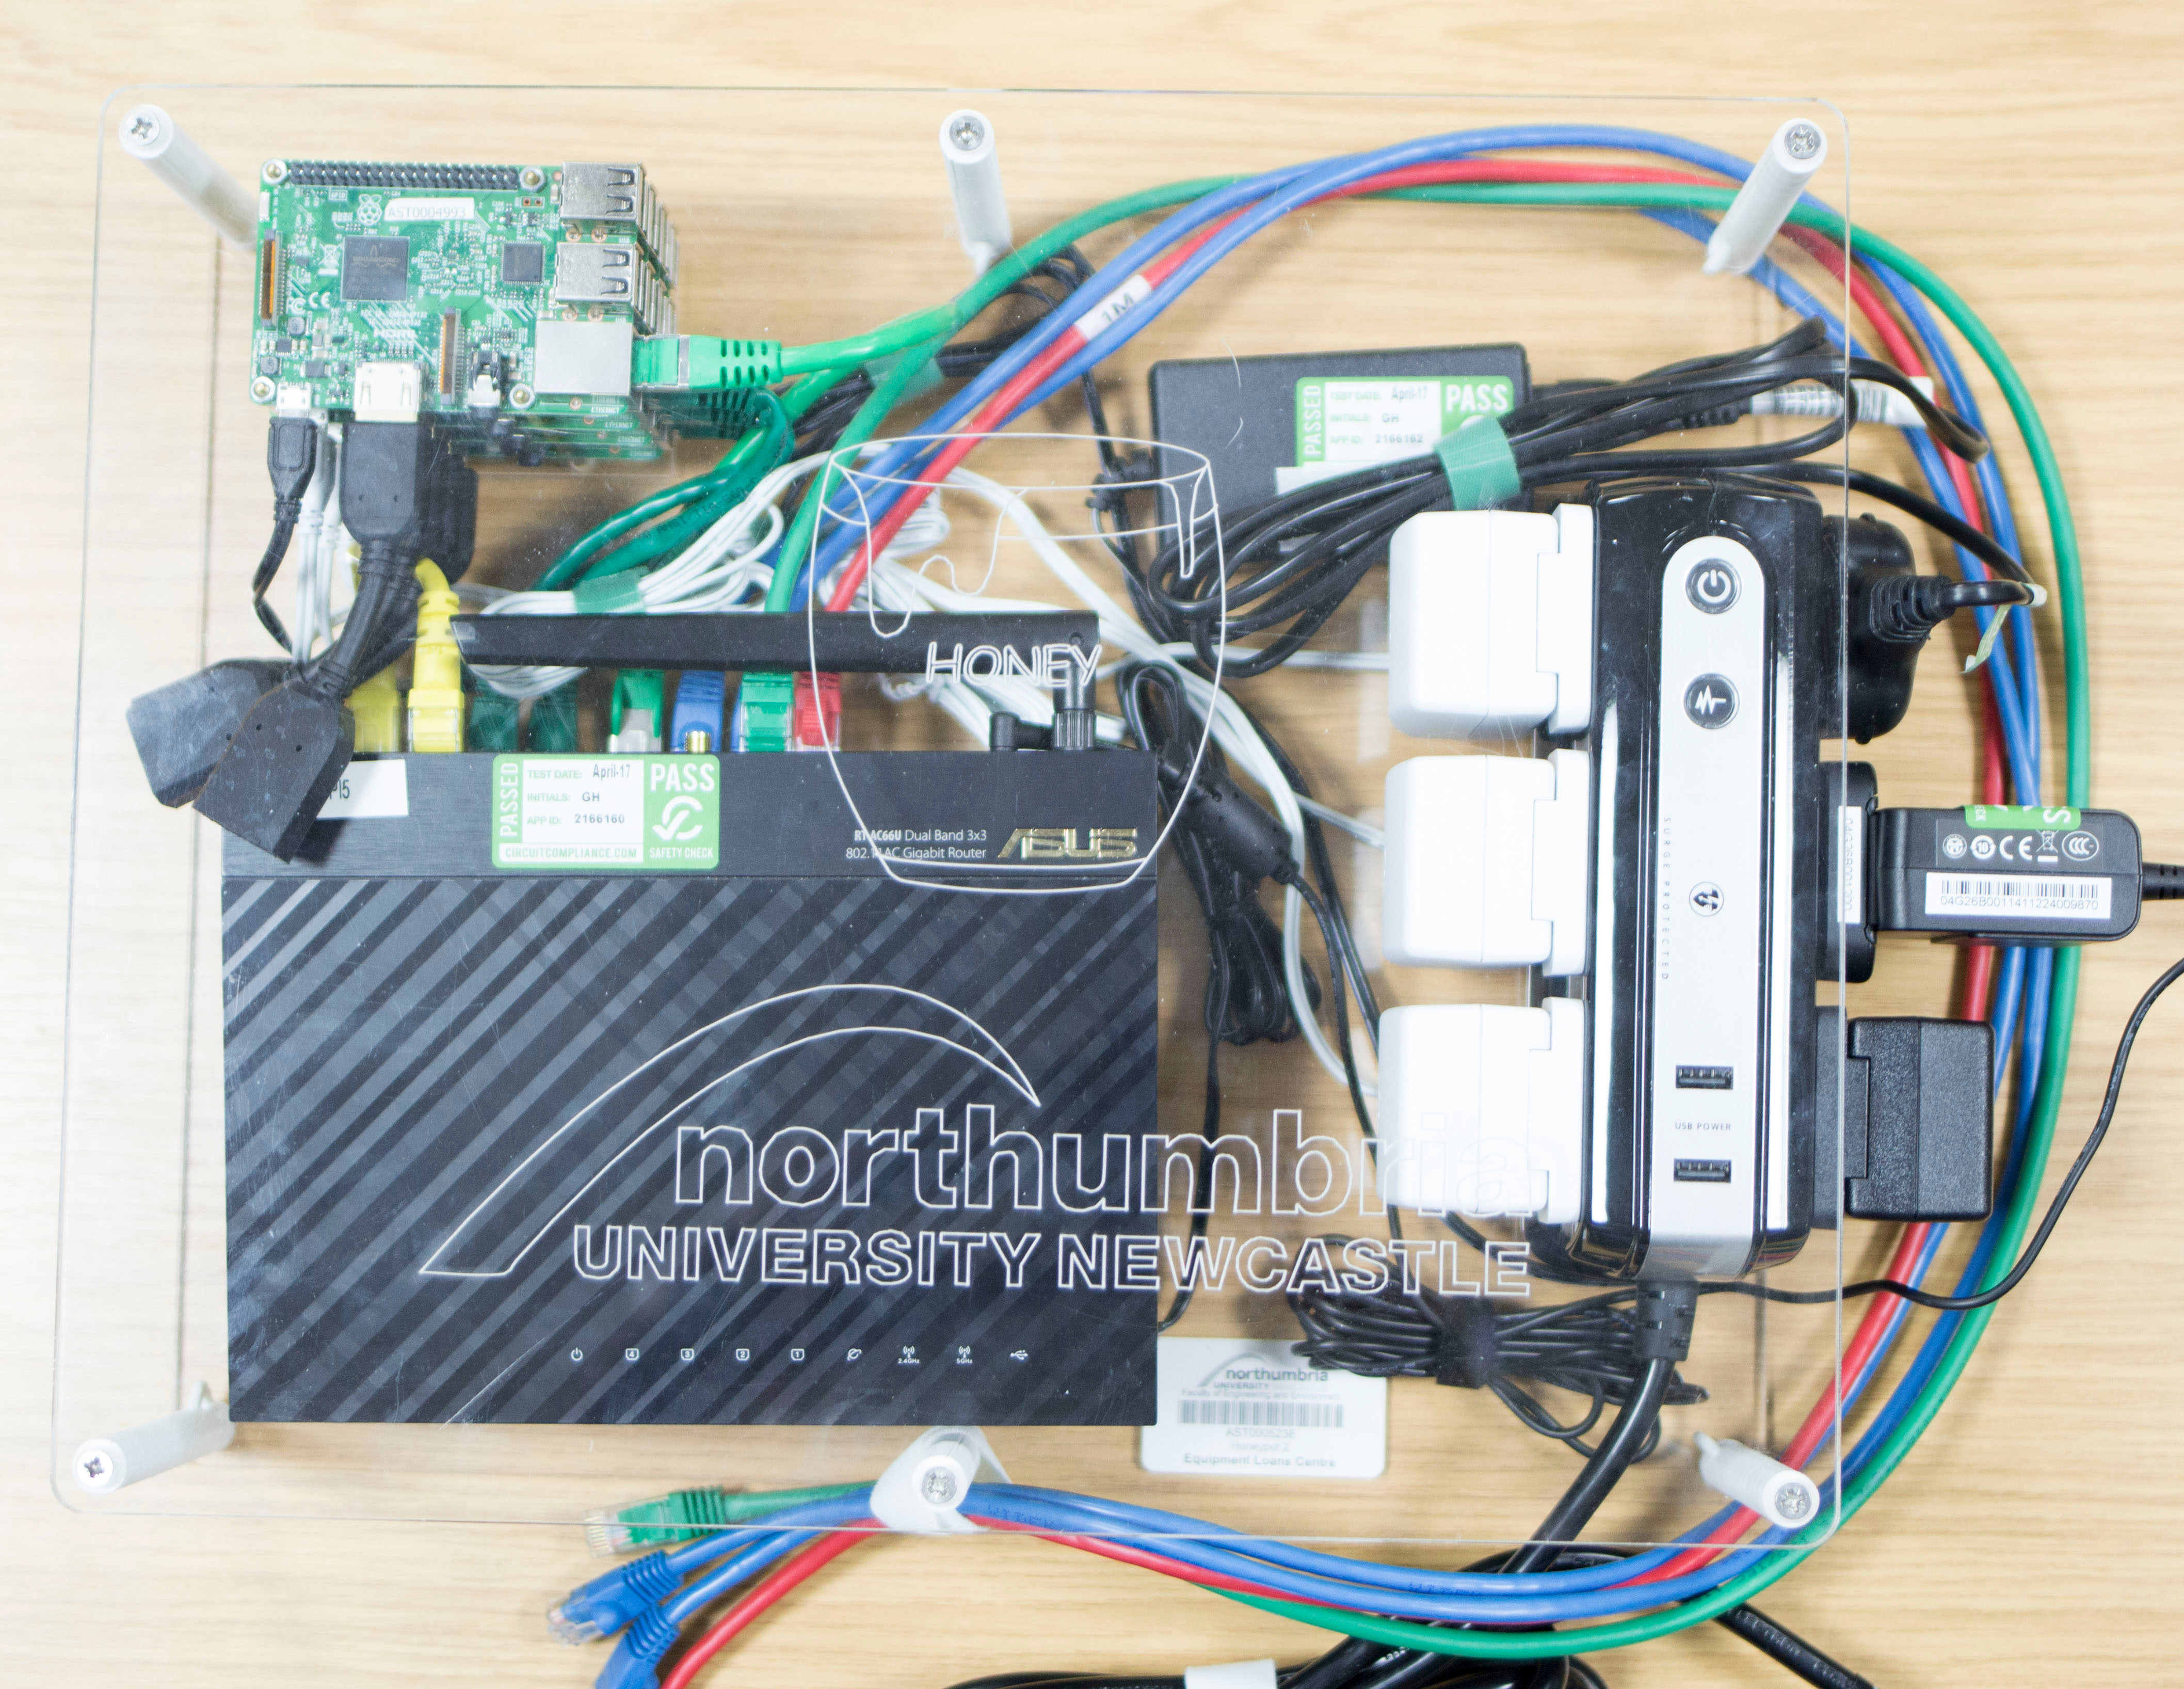
\includegraphics[width=\textwidth]{Images/HP2.eps}
    \caption{\texttt{HILV} top view\label{fig:HP2}}
  \end{minipage}
\end{figure}

%% \begin{figure}[htb]
%% \begin{center}
%% 	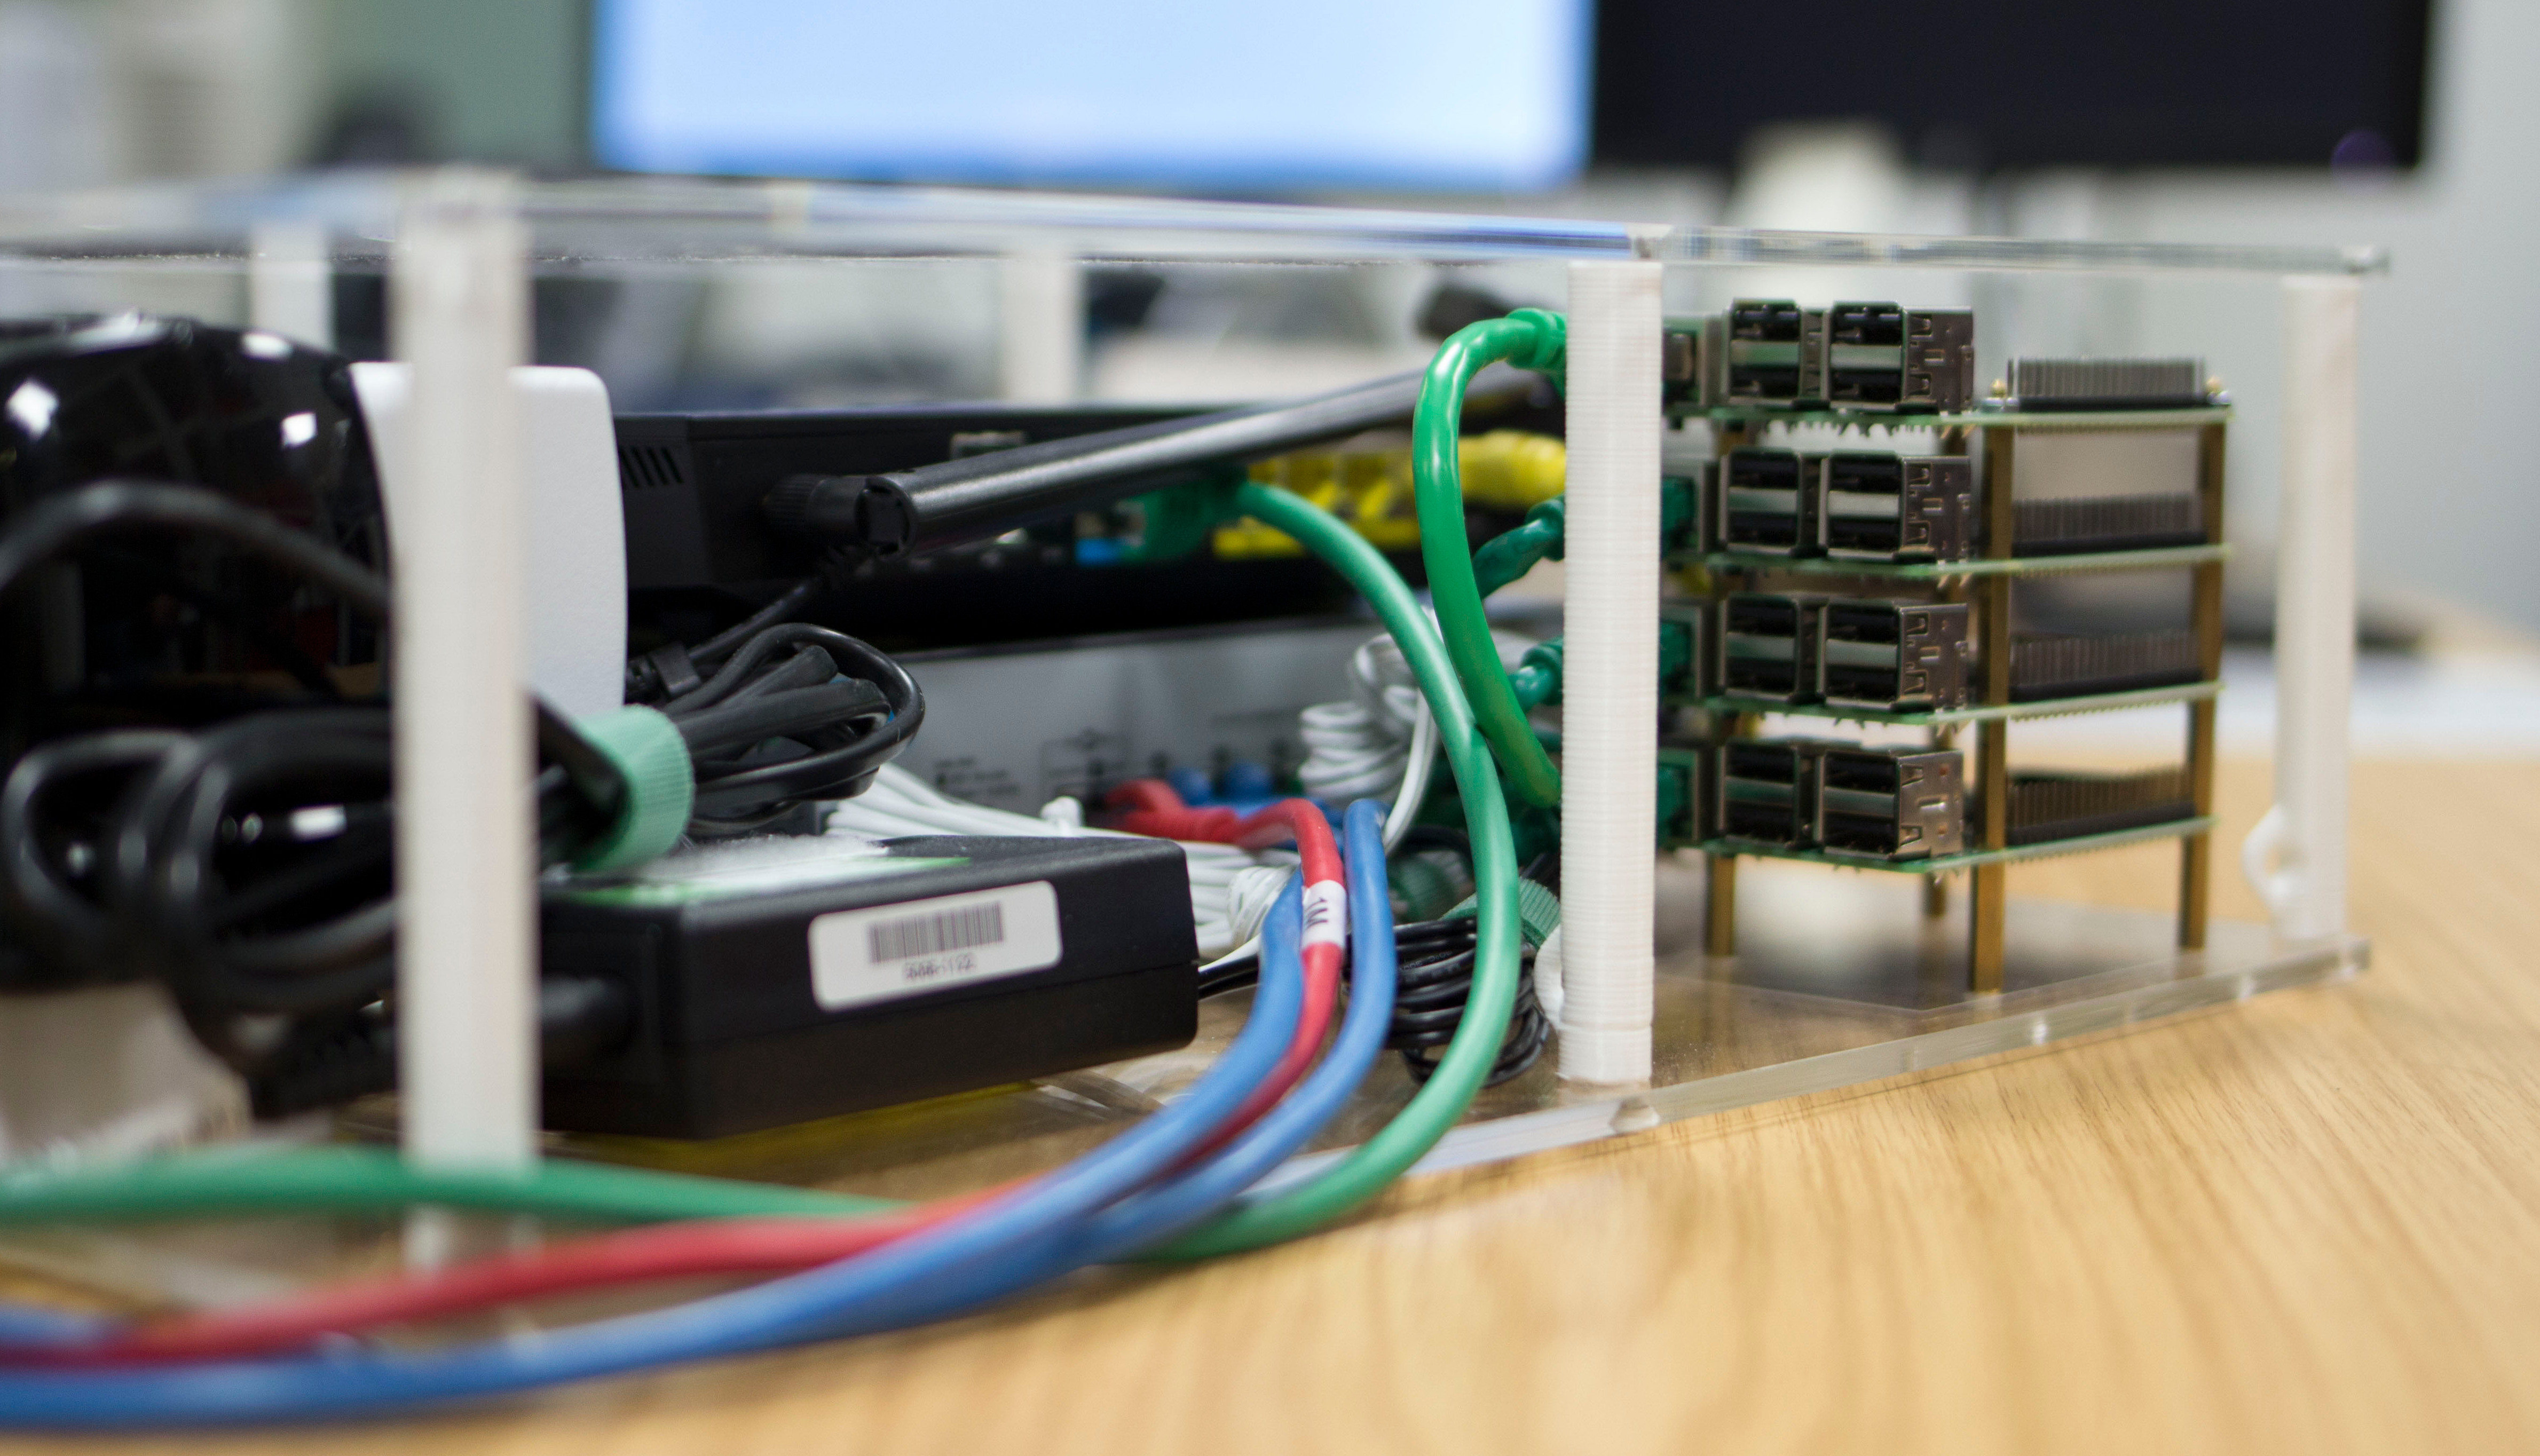
\includegraphics[scale=0.25]{Images/HP3.eps}
%% \caption{\texttt{HILV} Raspberry Pi boards (side view)}
%% \label{fig:HP3}
%% \end{center}
%% \end{figure}

Using Raspberry Pi boards as the main server technology within the honeypot has
allowed reconfiguration and rebuilding of the architecture to be simplified.
The operating system (and configured services) are stored on removable media
(micro SD cards) which simplifies server recovery and the maintaining of
multiple configurations. Images of the honeypot's base configuration can easily
be restored. Multiple configuration can be kept on different image sets and
students can keep individual projects as a set of micro SD cards that they
retain for the duration of a project.

\subsubsection{Address Range Support.}

The \texttt{HILV} honeypot environment must reside on a different subnet
address for the double \texttt{NAT}'d configuration to function correctly. This
is achieved by assigning a private, class A \texttt{IP} range providing more
than 16 million addresses.

\subsubsection{Router Configuration.}

The \texttt{HILV} honeypot's \texttt{ADSL} router is configured to provide only
routing services by disabling all other services for example \texttt{NAS} and
\texttt{DHCP} facilities. This configuration allows all infrastructure
protocols to be managed from within the honeypot using small scale servers
(Raspberry Pi boards~\cite{RASP:17}). Configuring the services on separate
servers allows analysis of inter-service activity during normal network
activity and during an attack.

The router used in the \texttt{HILV} honeypot is an ASUS RT
AC66U~\cite{ASUS:17}. The router is configured to use laboratory based
\texttt{DHCP} server to acquire an  address. The \texttt{IP} address is
allocated from a reservation which allows a consistent mapping of the forwarded
\texttt{IP} address from the Internet-based router to the research honeypot
router. Defining the mapping in this way allows external host names
(\texttt{URL}s) to be mapped to the honeypot for Internet-based attack
analysis. Forwarding of the traffic from the research router into the honeypot
can be enabled and disabled when required.

For direct access to the honeypot from the laboratory \texttt{IP} forwarding is
configured such that it will ``point'' to a target machine within the honeypot
as shown in Fig.~\ref{fig:Forward}. In small scale routers this operation is
normally referred to as a \texttt{DMZ} (demilitarised zone)
redirection~\cite{DK:08,MB:01}.

\begin{figure}[h]
\begin{center}
	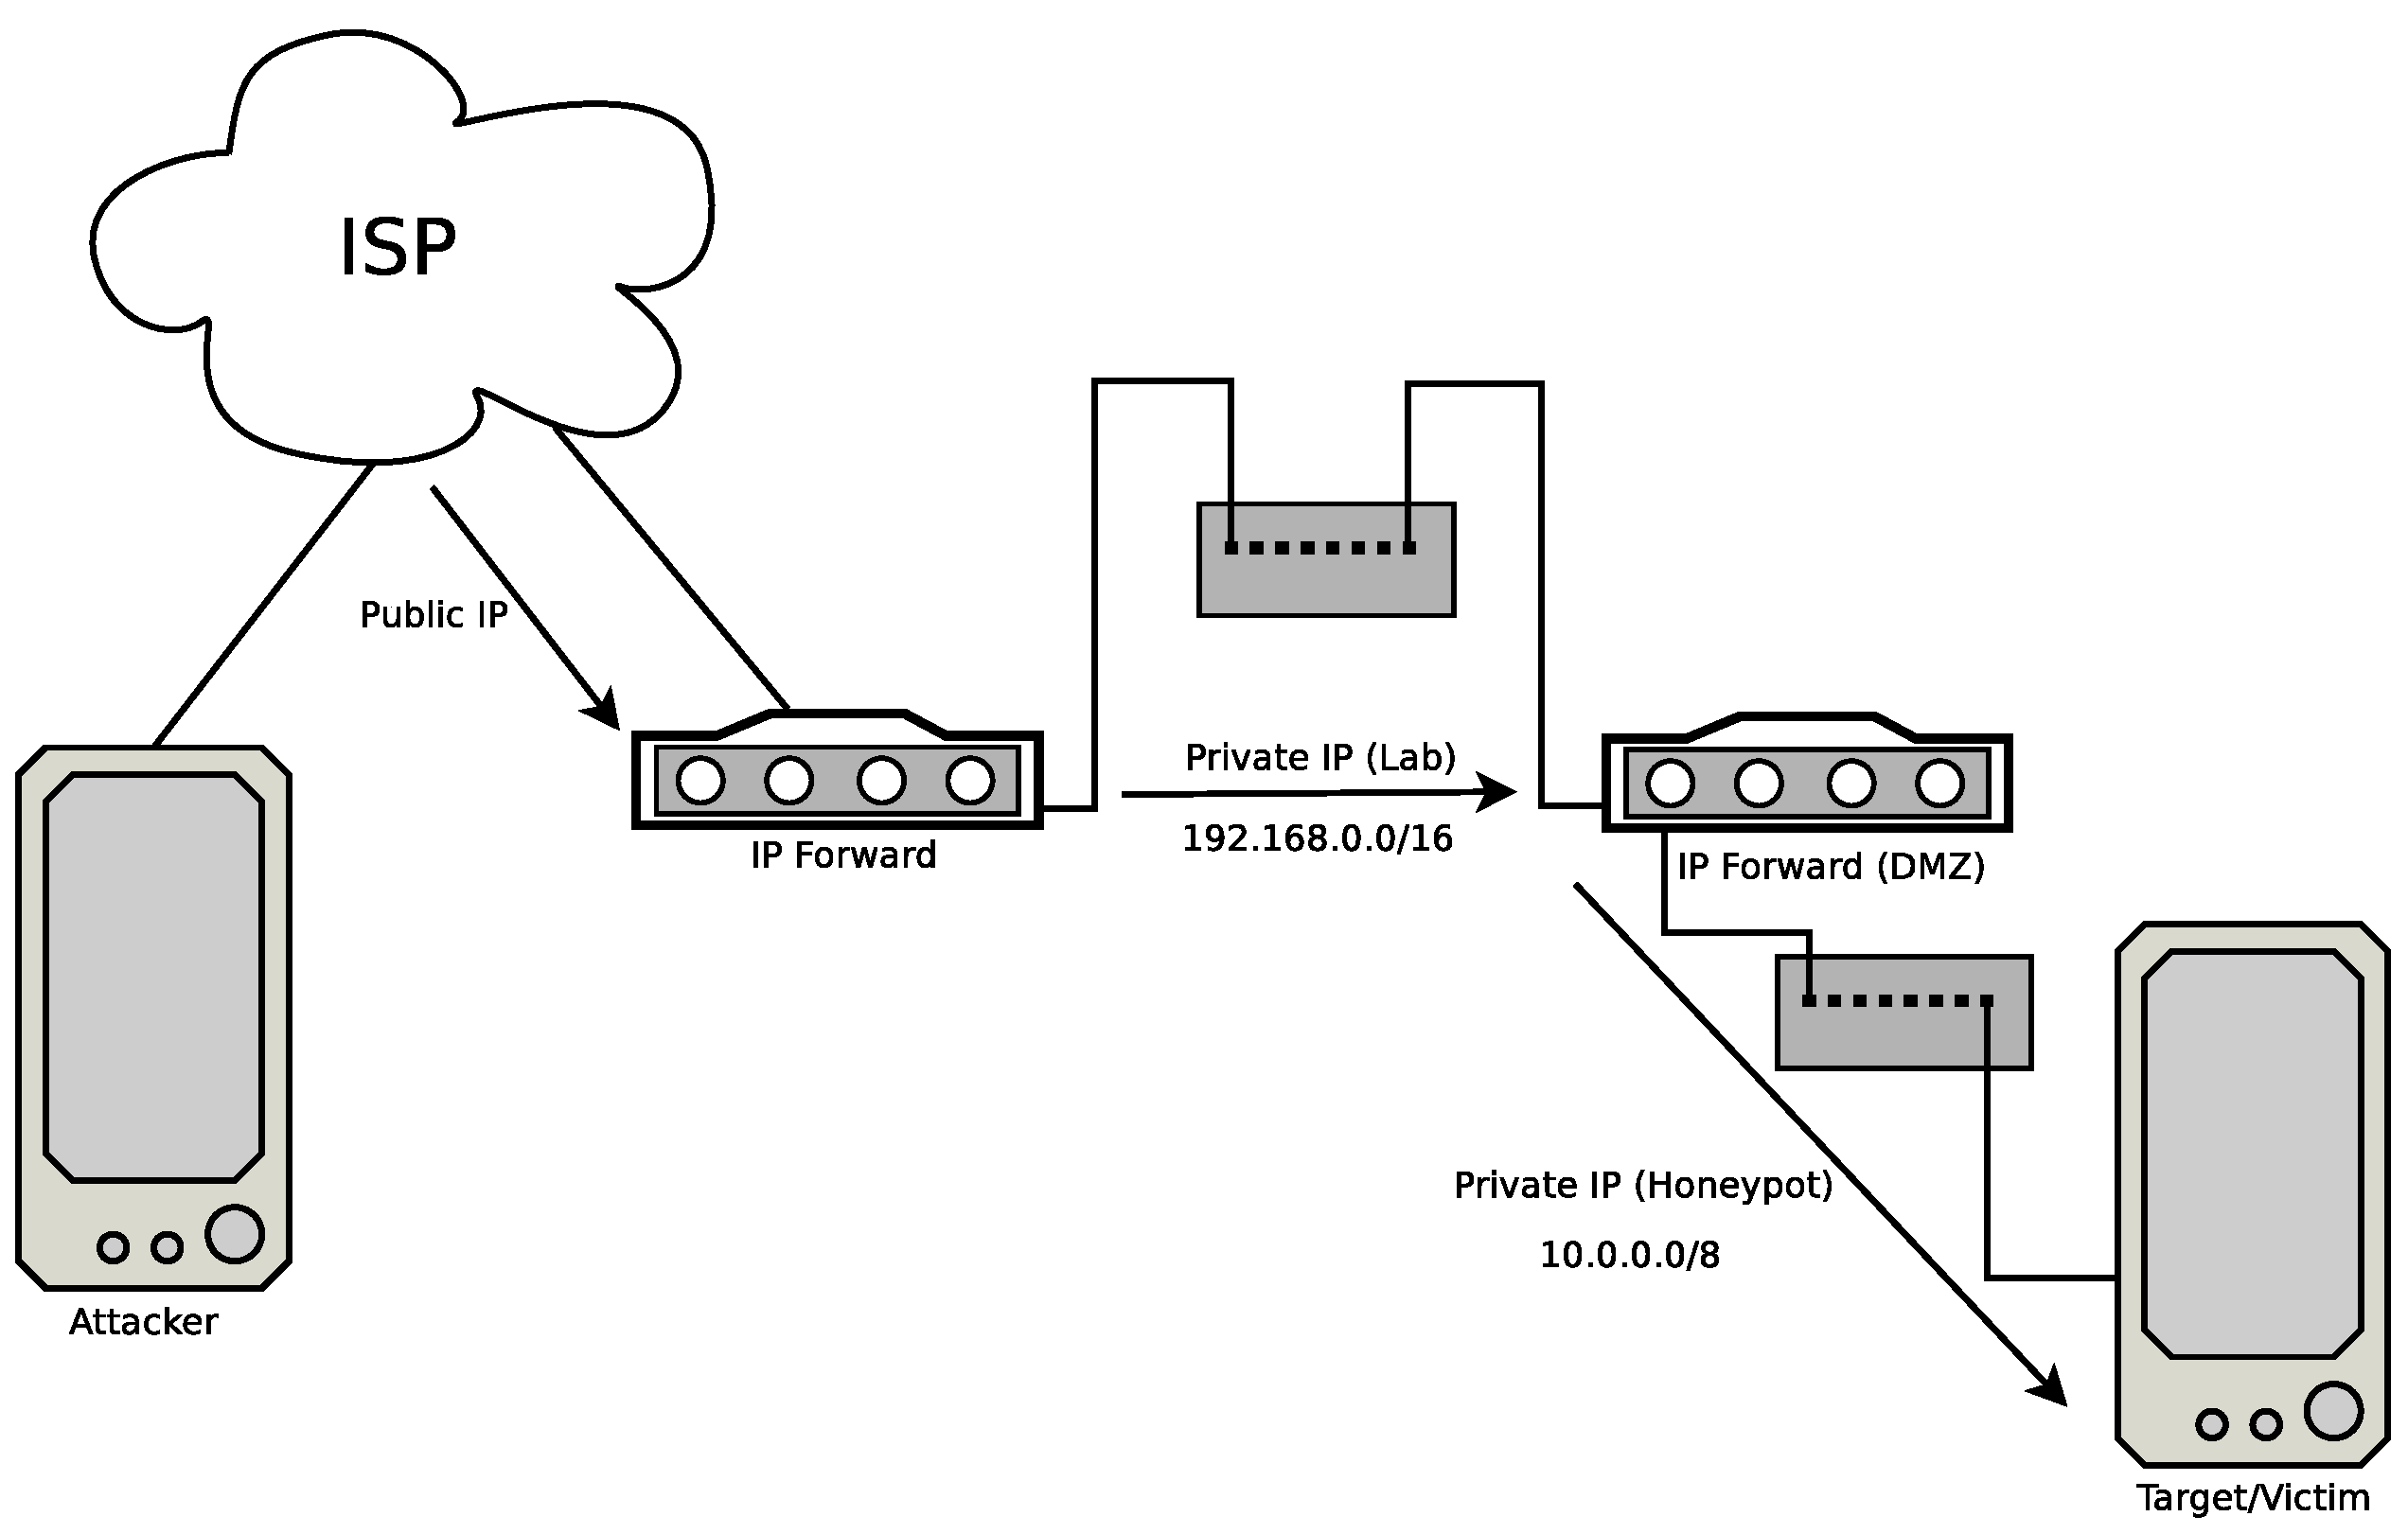
\includegraphics[scale=0.25]{Images/Forward.eps}
\caption{Address/Port forwarding}
\label{fig:Forward}
\end{center}
\end{figure}

\subsubsection{Switch Configuration.}

The main component of the \texttt{HILV} honeypot is a commercially available 8
port managed switch. The switch must support layer 2 management~\cite{ST:98} to
provide two specific technologies: port mirroring and port throttling. Suitable
switches include HP 2530-08~\cite{HP:17} or TP-LINK TL-SG2008~\cite{TP:17}.
Port mirroring and port throttling combined provided a reliable packet capture
architecture. 

\paragraph{Port mirroring.}
Switches by design provide a layer of security through virtual
circuits. A virtual circuit is an internal route whereby traffic is filtered by
the \texttt{Ethernet\_II} frame header. Switches maintain an in-memory table of
ports and \texttt{MAC} addresses to route each packet to a specific port. The
result of this routing is that packets are transferred port to port and not
broadcast, which limits packet capture. When using a Honeypot packet capture is
a vital part of the architecture for analysis of any network based attack
vector. Using a managed switch (as discussed above) it is possible to configure
the ports on the switch to be mirrored to a specific port as shown in
Figs.~\ref{fig:HPOverview} and~\ref{fig:throttling}. This allows all the
network activity to be captured and analysed~(\emph{Requirement 8}).

\paragraph{Bandwidth throttling.} 
A further issue with capturing the packets within the honeypot that must be
addressed is packet loss on the port where the mirrored traffic is forwarded.
Switches by design endeavour to provided the maximum transfer speed possible
between ports. This is achieved through the switch's backplane. The mirroring
of packets has a lower priority than that of throughput and therefore packet
loss on a mirrored port is inevitable on a heavily loaded switch. To prevent
this occurring the switch must be configured to throttle the throughput on the
mirrored ports so as not to overwhelm the backplane.
Figure~\ref{fig:throttling} shows the basic configuration of a throttled
environment. The port which has the packets forwarded to it must be configured
to run at a speed that exceeds the total bandwidth of the mirrored ports. The
effect of this is that as packets are transferred between ports they are
reliably replicated via the backplane to the monitor port. This configuration
satisfies \emph{requirement 8}.

\begin{figure}[h]
\begin{center}
	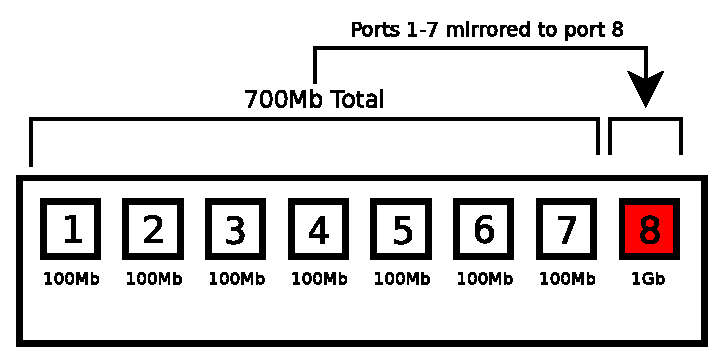
\includegraphics[scale=0.4]{Images/Throttle.eps}
\caption{Port throttling\label{fig:throttling}}
\end{center}
\end{figure}

Switches can implement mirroring in two ways. Firstly as a monitor-only port
where the transmission functionality of port is removed therefore no data can
be transmitted to the infrastructure (as in the case of an HP 1810-G). This
type of configuration therefore prevents a monitoring piece of equipment from
adding traffic to the network. Alternatively some manufacturers setup the
mirrored too port so it provided full functionality as well as the mirrored
capability (as in the case of a TP-SG2008). This allows the attached monitor to
also be used as a device within the honeypot. If the monitor port provides full
functionality the addition of a LAN tap~\cite{RB:13} can remove the
transmission facilities of the port creating the required monitor only
functionality as shown in Fig.~\ref{fig:HPOverview}.

\subsubsection{Internet Support.}

Access to the Internet from the honeypot is possible through the double
\texttt{NAT}'d configuration. The configuration provides isolation from the
laboratory and the Internet. Direct access to a target resource from the
Internet into either the laboratory based honeypot or into a small scale
research honeypot is achieved through packet forwarding as shown in
Fig.~\ref{fig:Forward}. For this technique to function correctly the
laboratory network and honeypot networks must be on different subnets.

The Internet facility also supports \texttt{IP} address forwarding to allow
Internet-based access into the research honeypots. From the Internet packets
are forwarded to the address of a honeypot router which is in turn forwards
traffic to a target machine inside the research honeypot as shown in
Fig.~\ref{fig:Forward}.

This configuration allows specific configurations to be exposed to capture
Internet-based attacks and to support remote access to the honeypot for remote
configuration and monitoring.

\subsection{\texttt{LIHV} Honeypot}

The \texttt{LIHV} is not intended for use in a reconfigurable environment and
does not require any monitoring or control of the network. No port monitoring
or throttling is required and all activity monitoring is achieved using log
file monitoring. The log files are made available on request for analysis of
service based access activity.

The \texttt{LIHV} honeypot is located in a separate cabinet, shown in
Fig.~\ref{fig:Overview2}. The cabinet is secured to prevent students having
direct access to the hardware. It supports the general service-base honeypot to
provide students with a platform to carry out simple authentication attacks
using tools such as \texttt{Hydra} from within the \texttt{Kali
Linux}~\cite{OS:17} toolset. This honeypot also provides a target for the
development of bespoke authentication attack tools in the final year
undergraduate cybersecurity modules.

\begin{figure}[h]
\begin{center}
	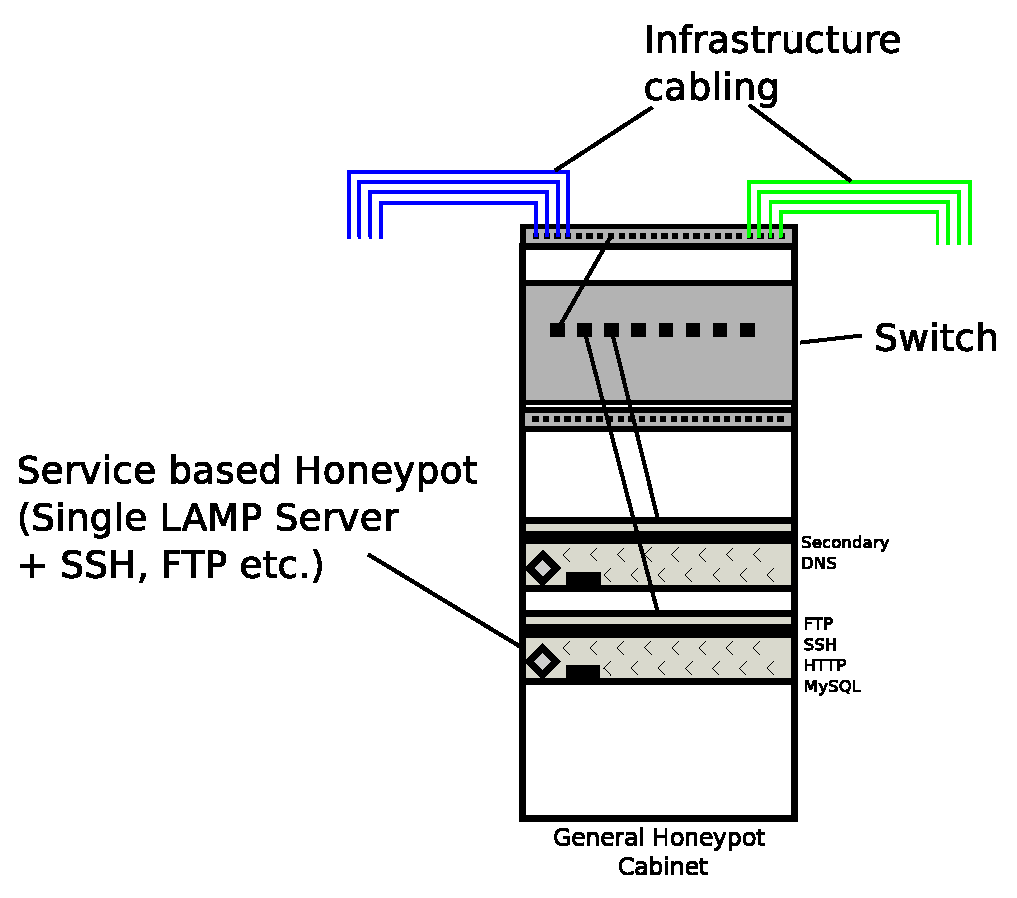
\includegraphics[scale=0.4]{Images/Infrastructure2.eps}
\caption{Laboratory general purpose honeypot overview}
\label{fig:Overview2}
\end{center}
\end{figure}

\subsubsection{Laboratory-Based Honeypot.}

The \texttt{LIHV} honeypot is a single 1U \texttt{LAMP} server
(Fig.~\ref{fig:Overview2}). This server is accessed directly in the
laboratory or via the Internet as a bastion server~\cite{MB:05} through
\texttt{IP} forwarding from the Internet router. The server is used primarily
for authentication attack projects based on dictionary attacks and scanning
based reconnaissance, for instance, with Nmap~\cite{GFL:09} or service analysis
tools such as WPScan~\cite{WT:17}. These types of attacks have a low impact on
the network as a whole and are therefore safe to run in the general purpose
laboratory. This machine is available internally and externally from the
laboratory to support directed learning tasks and also to support collaborative
ventures.

\section{Operational Results\label{Results}}

The base infrastructure has been in place, and actively used, for 10 years. The
laboratory-based honeypot has been in place for 9 years. The honeypot was
introduced to support the undergraduate networking program when the
cybersecurity module was introduced. This module was added to the BSc (Hons)
Ethical Hacking degree 7 years ago in 2010.

The (\texttt{LIHV}) honeypot has been successfully used in the teaching of
basic attack vectors such as port analysis, banner grabbing and service
interaction (\texttt{FTP} and \texttt{HTTP}) for modules and projects.

The (\texttt{HILV}) honeypots were designed and built 6 years ago and have been
used since 2012 (5 years) on both the undergraduate networking and ethical
hacking courses. The have been deployed in activities such as service
redirection attacks, amplification attacks and man-in-the-middle scenarios.

The (\texttt{HILV}) research honeypots using Raspberry Pi boards has allowed
diverse subjects to be taught more easily due to their use of removable media
to store the operating system. The setup time for laboratories and teaching
sessions has been dramatically reduced compared to using small clusters of PC's
with removable drives.

There have been several hardware changes to the (\texttt{HILV}) research
honeypots over this time but the basic architecture has remained unchanged. The
latest change was a Raspberry Pi 2 to Raspberry Pi 3 upgrade. The cost of layer
2 switches and their availability has also improved and are now more
affordable. As new honeypots are fabricated TP-LINK switches are being used in
reference to the more expensive HP switches. The TP-LINK switches do not
provide a fully implemented monitor port, this necessitates the need for the
inclusion of a network tap as shown in Fig.~\ref{fig:HPOverview}.

\subsection{Current Resource Support\label{ResourceSupport}}

The current implementation of the laboratory supports $>200$ students. This
includes undergraduate programs covering networking ($\sim40$), networking and
cybersecurity ($\sim150$) and postgraduate programmes covering networking
($\sim20$). Each of these programmes are modularised (broken down into
modules).  A typical undergraduate programme runs around $10$ modules
concurrently e.g.\ networking technology (years 1, 2, 3 \& 4 with MComp),
security case projects (Year 2), Sockets programming (year 3). Each module
requires $\sim3$ hours contact per week and $\sim3$ hours of directed learning,
which may require laboratory time. In addition the laboratory supports many
undergraduate and post graduate cybersecurity projects ($\sim80$) including
cyber attack analysis and general cybersecurity research such as
biometric-based multi-factor authentication and \texttt{IoT} (Internet of
Things) security projects.

\subsection{Supported Modules\label{Modules}}

All network engineering modules across both undergraduate and postgraduate
programmes involving routing, switching, \texttt{VLAN} deployment,
\texttt{MPLS} networking and \texttt{IP} telephony are all successfully taught
using the general networking laboratory infrastructure.

Network service deployment using server operating systems (Windows and Linux)
for both undergraduate and postgraduate programmes are taught successfully in
the environment using virtual machine technologies. The network service
deployments include load-balanced \texttt{HTTP}, network file system
deployments (\texttt{NFS} and \texttt{SMB}), replication based \texttt{MySQL}
services and large scale \texttt{DNS} deployments.

The \texttt{HILV} honeypot environment has allowed aspects of network based
infrastructure, specifically broadcast based network services, to be taught as
a practical implementation rather than simulations and has allowed students to
develop complete infrastructures integrated to the Internet.

Cybersecurity modules are predominantly taught using the research-honeypot
platform specifically when looking at attack vectors that require packet
spoofing or resource exhaustion through high volume traffic generation.

The \texttt{HILV} honeypots have also allowed analysis of live attacks from the
Internet without impacting on the local laboratory network. Activities such as
port scanning are passed through directly to the research honeypot without
exposing the laboratory infrastructure. Implementing multiple research
honeypots has allowed profiles of subnet scanning and attacks to be analysed by
students and have provided them with a rich environment for experimentation and
analysis.

\subsection{Supported Projects\label{Projects}}

The most prolific area of usage of the research honeypot platforms is in the
area of cybersecurity final year projects some of which are listed below:

\begin{itemize} 
  \item \noindent \emph{Multi-Tiered defence analysis of a simulated cyber
    attack.} This project involved configuring the research honeypots to
    support a \texttt{IPFire} (software based firewall technology) and
    investigating potential tunnelling techniques that could compromise a
    military grade network deployment.  
  \item \noindent \emph{Development of a small \texttt{IDS}.} This project
    involved developing a libpcap based application to run on one of the
    honeypot Raspberry Pi's (v3)~\cite{RASP:17} that could monitor network
    traffic to identify a \texttt{SYN} flood attack using a basic window based
    statistical analysis.  
    \item \noindent \emph{Attack on a secure \texttt{IoT} protocol} This
      project involved developing a network of \texttt{IoT} devices for
      environment analysis (temperature and humidity) and identify the
      encrypted traffic (\texttt{MQTT}) which was then attacked using a block
      decryption technique.  
    \item \noindent \emph{Development of an \texttt{IDS} for a full subnet
      \texttt{MitM} attack} This project involved developing a stateful based
      \texttt{IDS} using libpcap to identify spoofed \texttt{ARP} packets.  
    \item \noindent \emph{Development of a \texttt{DOS} tool that attempts to
      prevent detection from an \texttt{IDS}} This project involved developing
      a \texttt{RAW} sockets based application that crafted packets to
      replicate valid traffic within the subnet environment.  
     \item \noindent \emph{Analysis of a \texttt{DNS} amplification} This
       project involved configuring a vulnerable \texttt{DNS} environment and
       executing an attack and analysing the bandwidth effect of the network.
\end{itemize}

\section{Conclusion and Future Work\label{Future}}

The development of the \texttt{HILV} honeypot environment has proved successful
for both teaching and research. The cost of the deployment has been minimised
to such an extent that rather than the laboratory supporting a single honeypot
platform, which has to be reconfigured between sessions, the laboratory can now
support multiple honeypot deployments that are highly configurable and
portable.

As the \texttt{HILV} honeypots are small scale and low cost the equipment is
permanently configured for teaching purposes. Each \texttt{HILV} honeypot is
capable of supporting four students at a time to work on research based modules
and allows practical cybersecurity modules to be delivered more effectively.

Student numbers have risen sharply for cybersecurity-specific courses and the
use of the honeypots has allowed additional levels of cybersecurity to be
incorporated into existing network courses. This has had a strategic impact on
the University since the B.C.S. (British Computing Society) added
cybersecurity as a required part of its accreditation process.

The aim going forward is to increase the number of \texttt{HILV} honeypots to
accommodate the increasing number of students. Due to the architecture being
low cost this is an achievable goal. It is also envisaged that using this
technology the department will be able to expand its cybersecurity based
research by recruiting PhD students in the subject area to work on diverse
projects that will require significantly different honeypot configurations by
introducing a \texttt{HIHV} honeypot deployment. This deployment will consist
of several large scale servers along with commercial grade switches and routers
and large scale data capture facilities.

%\begin{acknowledgements}
%If you'd like to thank anyone, place your comments here
%and remove the percent signs.
%\end{acknowledgements}

\bibliographystyle{splncs}
\bibliography{honeypot}

\end{document}

